\documentclass[10pt]{beamer}

% mac版,texShop 中Typeset选择 XeLaTex 

%%%%%%%%%%%%%%%%%%%%%%%%%%%%%%%%%%%%%
\usepackage[slantfont,boldfont]{xeCJK}
%\input{xecjkfonts},CJKtextspaces
\setCJKmainfont{STKaiti}   % STFangsong 设置缺省中文字体
\setCJKmonofont{SimSun}   % 设置等宽字体
\setmainfont{Times} % 英文衬线字体
\setmonofont{Times} % 英文等宽字体
\setsansfont{Times} % 英文无衬线字体
%%%%%%%%%%%%%%%%%%%%%%%%%%%%%%%%%%%%%%

\mode<presentation> {
  %\usetheme{Madrid}
  %\usetheme{Singapore}
  \usetheme{Warsaw}
  \setbeamercovered{transparent}
 % \usefonttheme[onlymath]{serif}  
 \usefonttheme{professionalfonts}%{structurebold}
 % \usefonttheme[onlymath]{structurebold}
  \usecolortheme{rose}
}

\usepackage[english]{babel}
%\usepackage[latin1]{inputenc}

%\usepackage{times}
%\usepackage[T1]{fontenc}


%\usepackage{epsfig}
\usepackage{graphics}
\usepackage{color}
\usepackage{amsmath,amssymb,mathrsfs}
\usepackage{amsfonts,stmaryrd}
%\usepackage{thmmarks}
%\usepackage{}



\newcommand\frakfamily{\usefont{U}{yfrak}{m}{n}}
\DeclareTextFontCommand{\textfrak}{\frakfamily}
\def\diag{\mathrm{diag}}


\title[数值计算方法]{数值计算方法}
\subtitle{-插值}


\subject{Talks}

% If you have a file called "university-logo-filename.xxx", where xxx
% is a graphic format that can be processed by latex or pdflatex,
% resp., then you can add a logo as follows:

% \pgfdeclareimage[height=0.5cm]{university-logo}{university-logo-filename}
% \logo{\pgfuseimage{university-logo}}

%\pgfdeclareimage[height=0.5cm]{university-logo}{ncsu_logo}
%\logo{\pgfuseimage{university-logo}}

% Delete this, if you do not want the table of contents to pop up at
% the beginning of each subsection:
%\AtBeginSubsection[] {
%  \begin{frame}<beamer>
%    \frametitle{Outline}
%    \tableofcontents[currentsection,currentsubsection]
%  \end{frame}
%}

% If you wish to uncover everything in a step-wise fashion, uncomment
% the following command:

% \beamerdefaultoverlayspecification{<+->}


\setbeamertemplate{theorems}[numbered]
\setbeamertemplate{caption}[numbered]


\newtheorem{proposition}[theorem]{Proposition}

%%%%%%%%%%%%%%%%%%%%%%%%%%%
% REMARK-STYLE-ENVIRONMENTS %
%%%%%%%%%%%%%%%%%%%%%%%%%%%
\newcounter{remark}
% \numberwithin{theorem}{section}
\def\openrem#1#2{\refstepcounter{remark}\bigskip

{\noindent\bf#1~\theremark\if#2!{. }\else{ (#2).}\fi}
\it}
\def\thmskip{}
\newenvironment{remark}[1][!]{\openrem{Remark}{#1}}{\thmskip}

%%%%%%%%%%%%%%%%%%%%%%%%%%%%
%% AlGORITHM-STYLE-ENVIRONMENTS %
%%%%%%%%%%%%%%%%%%%%%%%%%%%%
\newcounter{algorithm}
% \numberwithin{theorem}{section}
\def\openalg#1#2{\refstepcounter{algorithm}\bigskip

{\noindent\bf#1~\thealgorithm\if#2!{. }\else{ (#2).}\fi}
\it}
\def\thmskip{}
\newenvironment{algorithm}[1][!]{\openrem{Algorithm}{#1}}{\thmskip}
%
%
%%%%%%%%%%%%%%%%%%%%%%%%%%%%
%% Result-STYLE-ENVIRONMENTS %
%%%%%%%%%%%%%%%%%%%%%%%%%%%%
%\newcounter{result}
%\def\openrem#1#2{\refstepcounter{result}\bigskip
%{\noindent \it \bfseries#1~\theremark\if#2!{. }\else{ (#2). }\fi}}
%\newenvironment{result}[1][!]{\openrem{Result}{#1}}{\qed}




%%%%%%%%%%%%%%%%%%%%%%%%%%%
%Redefine the Symbols%
%%%%%%%%%%%%%%%%%%%%%%%%%%%

\def\mathbi#1{\textbf{\em #1}}

% integrals
\def\dx{\,{\rm d}x}
\def\dxb{\,{\rm d}\boldsymbol{x}}
\def\dy{\,{\rm d}y}
\def\dt{\,{\rm d}t}
\def\ds{\,{\rm d}s}
\def\du{\,{\rm d}u}

\def\dr{\,{\rm d}r}
\def\dtheta{\,{\rm d}\theta}

\def\dd{{\rm d}}

\def\intOm{\int_{\Omega}}
\def\intbOm{\int_{\partial \Omega}}

% differences
\def\Dx{\Delta x}
\def\Dt{\Delta t}
\def\D{\Delta}


% operators
\def\Ls{\mathscr{L}}

% matirices
\def\Js{\mathscr{J}}


%fields%
\def\R{\mathbb{R}}
\def\N{\mathbb{N}}
\def\Z{\mathbb{Z}}

%Spaces%
\def\H{\mathbb{H}}
\def\L{\mathbb{L}}
\def\P{\mathbb{P}}


\def\U{\mathbb{U}}
\def\V{\mathbb{V}}
\def\W{\mathbb{W}}
\def\X{\mathbb{X}}
\def\Y{\mathbb{Y}}

\def\Cinfty{C^\infty}




%vectors%
\def\ab{\boldsymbol{a}}
\def\bb{\boldsymbol{b}}
\def\cb{\boldsymbol{c}}
\def\db{\boldsymbol{d}}
\def\eb{\boldsymbol{e}}
\def\fb{\boldsymbol{f}}
\def\gb{\boldsymbol{g}}
\def\hb{\boldsymbol{h}}
\def\nb{\boldsymbol{n}}
\def\rb{\boldsymbol{r}}
\def\sb{\boldsymbol{s}}


\def\ub{\boldsymbol{u}}
\def\vb{\boldsymbol{v}}
\def\wb{\boldsymbol{w}}
\def\xb{\boldsymbol{x}}
\def\yb{\boldsymbol{y}}
\def\zb{\boldsymbol{z}}

\def\Bb{\boldsymbol{B}}
\def\Cb{\boldsymbol{C}}
\def\Eb{\boldsymbol{E}}
\def\Fb{\boldsymbol{F}}
\def\Ib{\boldsymbol{I}}
\def\Kb{\boldsymbol{K}}
\def\Ob{\boldsymbol{O}}
\def\Qb{\boldsymbol{Q}}
\def\Rb{\boldsymbol{R}}
\def\Sb{\boldsymbol{S}}
\def\Ub{\boldsymbol{U}}
\def\Vb{\boldsymbol{V}}
\def\Wb{\boldsymbol{W}}
\def\Xb{\boldsymbol{X}}
\def\Yb{\boldsymbol{Y}}
\def\Zb{\boldsymbol{Z}}

%domains%
\def\Om{\Omega}
\def\bd{\partial}
\def\bOm{\bar{\Omega}}

%bold symbols%
\def\alphab{\boldsymbol{\alpha}}
\def\phib{\boldsymbol{\varphi}}

%energy%
\def\Jc{\mathcal{J}}
\def\Oc{\mathcal{O}}

%Greeks%
\def\vphi{\varphi}

%Special Functions%
\def\supp{\rm{supp}}
\def\sym{\rm{sym}}

\def\gradu{\nabla u}
\def\gradv{\nabla v}

%Mesh%
\def\Ts{\mathcal{T}}

\def\mach{\rm{mach}}


\begin{document}

\setbeamertemplate{itemize item}[triangle]

\begin{frame}
\titlepage
\end{frame}


\begin{frame}
  \frametitle{本节概要}
  \tableofcontents%[pausesections]
  % You might wish to add the option [pausesections]
%  \begin{itemize}
%  \item 显示Euler法及其误差分析
%  \item Taylor展开法
%  \item 
%  \end{itemize}
\end{frame}


\section{多项式插值及其误差估计}

\begin{frame}
\frametitle{插值概论}
有效表示数据是科学研究的一个基本的问题。实际问题中,数据点$(x,y)$可能是通过某个函数$y = f(x)$生成的,或者$(x,y)$是通过某种方法测量得到的,例如在化学反应中$x$表示温度$y$表示反应速率。

\vspace{0.2cm}

自变量$x$和$y$的关系包含了很多信息,但是我们希望在除了给定的点之外的点上也能够通过$x$的值计算出$y$的值,并且我们希望用简单的函数来表示这种关系以便我们可以用有限步的运算来计算出$y$的值。

\vspace{0.2cm}

下面我们开始讨论如何用多项式函数对给定数据进行插值,也就是说在给定数据点的情况下,我们如何寻找多项式使得这个多项式经过给定的数据点。


\end{frame}

\begin{frame}
\frametitle{插值}
\begin{definition}[插值]
如果一个函数$P(x)$经过给定的一个数据点的集合$(x_1, y_1), \ldots, (x_n,y_n)$,即$P(x_i) = y_i$,则我们说这个函数对这个集合的数据点进行了插值。
\end{definition}
例如给定的数据点的集合是$\{(0,1),(2,2),(3,4)\}$,则有一条抛物线$P(x) = \frac{1}{2}x^2 - \frac{1}{2}x+ 1$对这个数据点的集合进行了插值
\begin{figure}
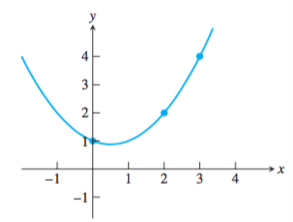
\includegraphics[width=4cm]{figs/3_1_Interp-1} 
\caption{点$(0,1),(2,2),(3,4)$被$P(x) = \frac{1}{2}x^2 - \frac{1}{2}x+ 1$插值} 
\end{figure}
\end{frame}


\begin{frame}
\frametitle{插值}
对于插值,我们有以下几点需要注意:
\begin{itemize}
\item 首先,由于$P(x)$是一个函数,因此对于插值点,我们必须有$x_i \neq x_j, i \neq j$。这是因为一个函数在给定一点上只能有一个值。当然,我们不要求$y_i \neq y_j, i \neq j$,因为函数可以在不同的点上等于相同的值。
\item 第二,我们将会只考虑多项式插值,这是因为,不论有多少的插值点,我们会发现,只要满足$x_i \neq x_j, i \neq j$,都会存在唯一的多项式$P(x)$使得$P(x_i) = y_i$。
\item 第三,使用多项式插值还有以下原因:首先,多项式有非常好的性质(例如可积性和可导性);其次,多项式求值只需要简单的加减乘除,而这些运算是计算机实际上唯一能做的,而且能够快速做的运算,所以多项式求值的速度实际上比一般函数求值要快得多。
\item 第四,我们可以把插值看作是多项式求值的逆运算。后者是给定函数和自变量,求函数在自变量点上的值,而前者是给定自变量和函数值,求满足要求的函数。
\end{itemize}
\end{frame}


\begin{frame}
\frametitle{拉格朗日插值多项式}
我们以三个数据点为例,假设我们有三个数据点$(x_1, y_1), (x_2, y_2), (x_3, y_3)$,则
\begin{equation}
P_2(x) = y_1 \frac{(x - x_2)(x - x_3)}{(x_1 - x_2)(x_1 - x_3)} + y_2 \frac{(x - x_1)(x - x_3)}{(x_2 - x_1)(x_2 - x_3)} + y_3 \frac{(x - x_1)(x - x_2)}{(x_3 - x_1)(x_3 - x_2)} 
\end{equation}
称为过这三个点的Lagrange插值多项式。

\vspace{0.2cm}

我们容易看到,当$x = x_1$时,多项式的后两项等于$0$(因为带分数线部分的分子为$0$),而第一项的
带分数线的部分为$1$,因此有$P_2(x_1) = y_1$。同理,我们有$P_2(x_2)  = y_2$以及$P_2(x_3)  = y_3$。
\end{frame}


\begin{frame}
\frametitle{拉格朗日插值多项式}
对于之前我们考虑的插值点过$\{(0,1),(2,2),(3,4)\}$的问题,如果利用Lagrange插值多项式构造,我们有
\begin{figure}
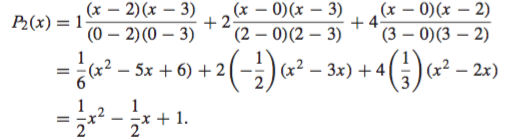
\includegraphics[width=8cm]{figs/3_1_1_Lagrange-1} 
%\caption{点$(0,1),(2,2),(3,4)$被$P(x) = \frac{1}{2}x^2 - \frac{1}{2}x+ 1$插值} 
\end{figure}
代入验证得$P_2(0) = 1, P_2(2) = 2, P_2(3) = 4$。 
\end{frame}


\begin{frame}
\frametitle{拉格朗日插值多项式的一般形式}
一般的,我们可以这样构造Lagrange插值多项式:考虑插值点$(x_1, y_1), \ldots, (x_n,y_n)$,对于$1 \le k \le n$,我们令Lagrange插值基函数$L_k(x)$满足
\begin{equation}
L_k(x) = \frac{(x - x_1) \cdots (x - x_{k-1}) (x - x_{k+1}) \cdots (x- x_n)}{(x_k - x_1) \cdots (x_k - x_{k-1})(x_k - x_{k+1}) \cdots (x_k - x_n)}.
\end{equation}
容易验证,$L(x)$满足$L_k (x_k) = 1$而$L_k(x_j) = 0, j \neq k$。进而,我们令
\begin{equation}
P_{n-1}(x) = y_1 L_1(x) + \cdots + y_n L_n(x),
\end{equation}
容易验证
\begin{align}
P_{n-1}(x_k) & = y_1 L_1(x_k) +\cdots  + y_k L_k(x_k)+ \cdots + y_n L_n(x) \nonumber \\
                     & = 0 +\cdots  + y_k + \cdots + 0 \nonumber \\
                     & = y_k.
\end{align} 
\end{frame}


\begin{frame}
\frametitle{拉格朗日插值多项式的唯一性}
通过以上的过程我们构造出了满足插值条件的多项式,而非常有趣的是,我们可以证明这个插值多项式是唯一的。
\begin{theorem}[多项式插值定理]
给定$n$个插值点$(x_1, y_1), \ldots, (x_n,y_n)$,满足$x_i \neq x_j, i \neq j$,存在唯一的小于等于$n-1$阶插值多项式$P$满足$P(x_i) = y_i, i = 1, \ldots, n$。
\end{theorem}

\begin{remark}
以上定理只是告诉我们,给定满足条件的$n$个插值点的次数不超过$n-1$次的多项式是唯一的,那么一方面,如果多项式次数可以超过$n-1$次的话,那么就可能有多个插值多项式满足条件,另一方面,这个唯一的插值多项式的次数不一定就是$n-1$,比如过三个在同一直线上的次数不超过$2$次的插值多项式就是一次的。
\end{remark}
\end{frame}


\begin{frame}
\frametitle{插值多项式的另一种导出}
Lagrange插值多项式给出了插值多项式的一种构造性的构建方法。现在我们提出这样一个问题:数据点增加了一个$(x_{n+1}, y_{n+1})$之后,如何构造新的插值多项式?

\vspace{0.2cm}

如果我们仍然用Lagrange插值法,则我们必须首先构造新的Lagrange插值基函数,再构造插值多项式。这个过程是十分麻烦的。因此我们考虑能否利用已经得到的插值多项式来构造新的插值多项式。

\vspace{0.2cm}

这是可以实现的。例如我们首先考虑插值点$(0,1), (2,2)$,则容易得到插值函数就是过这两点的直线方程
\begin{equation}
P_1 (x)= \frac{1}{2} x + 1.
\end{equation}
现在新增了插值点$(3,4)$,我们考虑如下形式的函数
\begin{equation}
P_2(x) = P_1(x) + cx(x-2).
\end{equation}
容易看到,$P_2(0) = P_2(2) =0$
\end{frame}


\begin{frame}
\frametitle{插值多项式的另一种导出}
现在新增了插值点$(3,4)$,我们假设新的插值函数$P_2(x)$满足
\begin{equation}
P_2(x) = P_1(x) + cx(x-2).
\end{equation}
容易得到,
\begin{equation}
P_2(0) = P_1(0) + 0 = 1, P_2(2) = P_1(2) + 0 = 2.
\end{equation}
现在令$x = 3$,由于我们假设$P_2(x)$过插值点$(3,4)$,所以我们有
\begin{align}
4 = P_2(3) & = P_1(3) + c3\times(3-2) \nonumber \\
               c & = \frac{4 - \frac{5}{2}}{3} = \frac{1}{2}.
\end{align}
因此,满足插值条件的$P_2(x)$为
\begin{equation}
P_2(x) = \frac{1}{2} x(x-2) + P_1(x) =  \frac{1}{2} x(x-2) + \frac{1}{2} x + 1 =  \frac{1}{2} x^2 - \frac{1}{2} x + 1
\end{equation}
\end{frame}


\begin{frame}
\frametitle{插值多项式的另一种导出}
以上的推导实际上给出了一种计算插值多项式的有效算法。如果把以上的算法进行推广,对于$n$个插值点$(x_1, y_1), \ldots, (x_n,y_n)$,我们可以设插值函数$P_{n-1}(x)$满足
\begin{equation}
P_{n-1}(x) = a_0 + a_1(x - x_1) + a_2(x - x_1)(x-x_2)+ \ldots + a_{n-1}(x - x_1) \cdots (x - x_{n-1}).
\end{equation}
根据插值条件
\begin{align}
y_1 &= P_{n-1}(x_1) = a_0 \nonumber \\
y_2 &= P_{n-1}(x_2) = a_0 + a_1(x_2 - x_1) \nonumber \\
y_3 &= P_{n-1}(x_3) = a_0 + a_1(x_3 - x_1) + a_2(x_3 - x_1)(x_3 - x_2) \nonumber \\
&\vdots \nonumber \\
y_n &=  P_{n-1}(x_n) = a_0 + a_1(x_n - x_1) + a_2(x_n - x_1)(x_n  - x_2) + \ldots \nonumber \\
       & \quad \quad \quad  \quad \quad \quad + a_{n-1}(x_n - x_1) \cdots (x_n - x_{n-1}).
\end{align}
\end{frame}


\begin{frame}
\frametitle{系数的规律}
通过解以上关于$a_0, \ldots, a_{n-1}$的方程,我们可以得到以下规律
\begin{align}
a_0   & = y_1 \nonumber \\
a_1   & = \frac{y_2 - y_1}{x_2 - x_1}  \nonumber \\
a _2  & = \frac{1}{x_3 - x_2} \big\{\frac{y_3 - y_1}{x_3 - x_1} -   a_1\big\} \nonumber \\
         & =  \frac{1}{x_3 - x_2} \big\{\frac{y_3 - y_1}{x_3 - x_1} -    \frac{y_2 - y_1}{x_2 - x_1} \big\} \nonumber \\
a_3  & = \frac{1}{x_4 - x_3} \big\{ \frac{\frac{y_4 - y_1}{x_4 - x_1} -   a_1}{x_4 - x_2}  - a_2 \big\}  \nonumber \\
&\vdots
\end{align}
\end{frame}


\begin{frame}
\frametitle{差商的定义}
\begin{definition}[差商]
我们令$y_i = f[x_i], i = 1 \ldots n$为函数$f(x)$的零阶差商;
\begin{equation}
f[x_i, x_j] = \frac{f(x_i) - f(x_j)}{x_i - x_j}, i ,j = 1, \ldots, n, i \neq j
\end{equation}
为函数$f(x)$的一阶阶差商;
\begin{equation}
f[x_i, x_j,x_k] = \frac{f[x_j ,x_k] - f[x_i, x_j]}{x_k - x_i}, i ,j ,k= 1, \ldots, n, j \neq k
\end{equation}
为函数$f(x)$的二阶阶差商;
以及一般的
\begin{equation}
f[x_{i_1}, x_{i_2}, \cdots, x_{i_{k+1}}] = \frac{f[x_{i_2}, x_{i_3}, \cdots, x_{i_{k+1}}] - f[x_{i_1}, x_{i_2}, \cdots, x_{i_{k}}]}{x_{i_{k+1}} - x_{i_1}}
\end{equation}
为函数$f(x)$的$k$阶差商。
\end{definition}
\end{frame}


\begin{frame}
\frametitle{差商的性质}
可以证明差商有以下重要性质:
\begin{lemma}[差商的对称性]
差商具有对称性
\begin{equation}
f[x_1, \ldots, x_k] = f[x_{i_1}, x_{i_2}, \ldots, x_{i_k}],
\end{equation}
其中$i_1, \ldots, i_k$是$1, 2, \ldots, k$的任意一种排列。
\end{lemma}
\end{frame}

\begin{frame}
\frametitle{系数的差商表示}
根据上面系数的表达式以及差商的定义,我们又可以得到,
\begin{align}
a_0   & = y_1 = f[x_1]\nonumber \\
a_1   & = f[x_2, x_1] = \frac{f[x_2] - f[x_1]}{x_2 - x_1} \nonumber \\
a _2  & = f[x_1, x_2, x_3] = \frac{f[x_2,x_3] - f[x_1,x_2]}{x_3 - x_1}   - \nonumber \\
a_3   & = f[x_1, x_2 , x_3, x_4] = \frac{f[x_2,x_3,x_4] - f[x_1,x_2,x_3]}{x_4 - x_1}  \nonumber \\
&\vdots \nonumber\\
a_{n-1} & = f[x_1, \ldots, x_n] = \frac{f[x_2,\ldots,x_n] - f[x_1,\ldots,x_{n-1}]}{x_n - x_1}.
\end{align}
\end{frame}


\begin{frame}
\frametitle{牛顿差商表}
以上系数的差商表示让我们求多项式$P_{n-1}$的系数变得极为方便,在实际计算中,这种方便一般通过构造差商表来实现。例如对于三个点的插值问题,我们可以构造形式如下的牛顿差商表
\begin{figure}
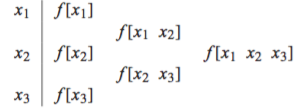
\includegraphics[width=5cm]{figs/3-1-2_Newton-1} 
%\caption{点$(0,1),(2,2),(3,4)$被$P(x) = \frac{1}{2}x^2 - \frac{1}{2}x+ 1$插值} 
\end{figure}

\begin{example}
利用牛顿差商表来计算过$\{(0,1),(2,2),(3,4)\}$的次数不高于二次的插值多项式。
\end{example}
\end{frame}


\begin{frame}
\frametitle{牛顿差商表}
利用牛顿差商表,得到
\begin{figure}
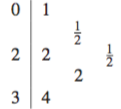
\includegraphics[width=2cm]{figs/3-1-2_Newton-2} 
%\caption{点$(0,1),(2,2),(3,4)$被$P(x) = \frac{1}{2}x^2 - \frac{1}{2}x+ 1$插值} 
\end{figure}
从而可得插值多项式
\begin{equation}
P_2(x) = 1 + \frac{1}{2}(x-0) + \frac{1}{2}(x-0)(x-2) =  \frac{1}{2} x^2 - \frac{1}{2} x + 1.
\end{equation}
\end{frame}


\begin{frame}
\frametitle{牛顿差商表}
如果这时我们再增加一个插值点$(1,0)$,则我们只需要在原来的差商表下方增加一行,得到新的差商表
\begin{figure}
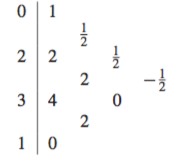
\includegraphics[width=3cm]{figs/3-1-2_Newton-3} 
%\caption{点$(0,1),(2,2),(3,4)$被$P(x) = \frac{1}{2}x^2 - \frac{1}{2}x+ 1$插值} 
\end{figure}
从而可得插值多项式
\begin{align}
P_3(x) & = 1 + \frac{1}{2}(x-0) + \frac{1}{2}(x-0)(x-2) - \frac{1}{2}(x-0)(x-2)(x-3) \nonumber \\
           & =  P_2(x) - \frac{1}{2}(x-0)(x-2)(x-3).
\end{align}
\end{frame}


\begin{frame}
\frametitle{插值多项式的快速计算方法}
事实上,上面的方法不光为我们提供了一个快速构造插值多项式的方法,利用上面的插值多项式我们还可以快速的进行插值多项式求值,这是因为上面的插值多项式的形式方便的让我们定义一个广义的秦九韶算法。

\vspace{0.2cm}

例如对于之前的$P_2(x)$,我们有
\begin{equation}
P_2(x) = 1 + \frac{1}{2}(x-0) + \frac{1}{2}(x-0)(x-2) = 1 + (x-0)[\frac{1}{2} + \frac{1}{2}(x-2)].
\end{equation}
而对于一般的$P_{n-1}(x)$,我们有
\begin{align}
P_{n-1}(x) & = a_0 + a_1(x - x_1) + a_2(x - x_1)(x-x_2)+ \ldots \nonumber \\
                 &\quad + a_{n-1}(x - x_1) \cdots (x - x_{n-1}) \nonumber \\
                 & = a_0 + (x-x_1)(a_1 + (x-x_2)(a_2 +\nonumber \\
                 & \quad  (\ldots (a_{n-2} + a_{n-1}(x-x_{n-1})) \ldots ))).
\end{align}
容易得到,利用Lagrange插值多项式计算多项式在某点的值的计算量为$O(n^2)$而牛顿差商法只需要$O(n)$。
\end{frame}


\begin{frame}
\frametitle{插值多项式的应用}
插值多项式的一个重要的应用是将计算复杂的函数的求值转变为多项式求值。典型的一个例子就是三角函数。

\vspace{0.2cm}

例如我们对$f(x) = \sin x$在$[0,\frac{\pi}{2}]$上的等距的四个点上进行插值。首先由牛顿差商法,得到差商表
\begin{figure}
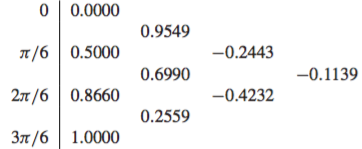
\includegraphics[width=5cm]{figs/3-1-5_sin-1} 
%\caption{点$(0,1),(2,2),(3,4)$被$P(x) = \frac{1}{2}x^2 - \frac{1}{2}x+ 1$插值} 
\end{figure}
则插值得到的三次多项式为
\begin{figure}
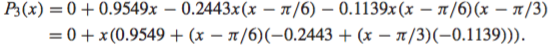
\includegraphics[width=9cm]{figs/3-1-5_sin-2} 
%\caption{点$(0,1),(2,2),(3,4)$被$P(x) = \frac{1}{2}x^2 - \frac{1}{2}x+ 1$插值} 
\end{figure}
\end{frame}


\begin{frame}
\frametitle{插值多项式的应用}
插值多项式$P_3(x)$与$\sin x$的比较图像如下
\begin{figure}
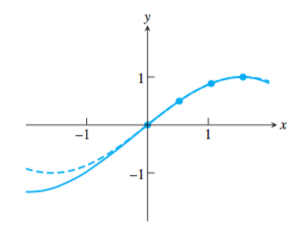
\includegraphics[width=5cm]{figs/3-1-5_sin-3} 
\caption{实线为插值多项式的图像;虚线为$\sin x$的图像} 
\end{figure}
\end{frame}


\begin{frame}
\frametitle{插值多项式的应用}
利用插值多项式以及$\sin (x)$的周期性计算$x$在各点的值见下表
\begin{figure}
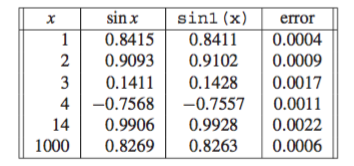
\includegraphics[width=6cm]{figs/3-1-5_sin-4} 
%\caption{点$(0,1),(2,2),(3,4)$被$P(x) = \frac{1}{2}x^2 - \frac{1}{2}x+ 1$插值} 
\end{figure}
可以看到,插值多项式的值与原函数的值是有误差的,虽然这里看起来不是很大,但是我们需要对这个误差作一个比较准确的估计,因此我们需要进一步讨论插值误差估计的问题。
\end{frame}


\begin{frame}
\frametitle{插值误差}
假设插值点$(x_1, y_1), \ldots, (x_n,y_n)$是由某个函数$f(x)$生成的,即$f(x_i) = y_i$,则我们有以下的插值误差表达式。

\begin{theorem}[插值误差]
\label{thm: interp error}
令$P(x)$是经过插值点$(x_1, y_1), \ldots, (x_n,y_n)$的$n-1$次多项式插值函数,假设这些插值点是由函数$f(x)$生成的且$f(x)$有$n$阶连续导数,则存在插值误差满足
\begin{equation}
f(x) - P(x) = \frac{(x - x_1)(x - x_2) \ldots (x-x_n)}{n!}f^{(n)}(\xi)
\end{equation}
其中$\xi$是$x, x_1, \ldots, x_n$中最大的数与最小的数之间的某个数。
\end{theorem}
\end{frame}


\begin{frame}
\frametitle{插值误差估计}
定理\ref{thm: interp error}给出了插值误差的表达式,但是由于$\xi$这个常数是不确定的,所以我们无法利用这个表达式来求得准确的误差。这个插值误差估计一般的使用方式是找到$f^{(n)}(x)$在由$x, x_1, \ldots, x_n$中最大的数与最小的数构成的区间上的绝对值的最大值,即找到$M = \max_{x \in [a,b]} |f^{(n)}(x)|$,进而得到
\begin{equation}
|f(x) - P(x)| \le |\frac{(x - x_1)(x - x_2) \ldots (x-x_n)}{n!}|M.
\end{equation}
\end{frame}


\begin{frame}
\frametitle{插值误差估计}
例如我们在之前的例子当中利用三次多项式对$f(x) = \sin x$在$0, \frac{\pi}{6}, \frac{2\pi}{6}, \frac{3\pi}{6}$四个点上进行插值。利用插值误差公式,对任意的$x \in [0, \frac{\pi}{2}]$,我们有
\begin{equation}
\sin x - P(x) = \frac{(x-0)(x- \frac{\pi}{6})(x-\frac{\pi}{3})(x- \frac{\pi}{2})}{4!}f''''(\xi),
\end{equation}
其中$\xi \in [0,  \frac{\pi}{2}]$。由于$f''''(x) = \sin x$,而$|\sin x| \le 1$,因此我们有
\begin{equation}
|\sin x - P(x)| \le \frac{|\frac{(x-0)(x- \frac{\pi}{6})(x-\frac{\pi}{3})(x- \frac{\pi}{2})}{4!}|}{24} |1|.
\end{equation}
\end{frame}


\begin{frame}
\frametitle{插值误差估计}
在$x =1$时,误差估计为
\begin{equation}
| \sin 1 - P(1) | \le \frac{|\frac{(1-0)(1- \frac{\pi}{6})(1-\frac{\pi}{3})(1- \frac{\pi}{2})}{4!}|}{24} |1| \approx 0.0005348
\end{equation}
而在$x = 0.2$时,误差估计为
\begin{equation}
| \sin 0.2 - P(0.2) | \le \frac{|\frac{(0.2-0)(0.2- \frac{\pi}{6})(0.2-\frac{\pi}{3})(0.2- \frac{\pi}{2})}{4!}|}{24} |1| \approx 0.00313.
\end{equation}
注意两个问题:
\begin{itemize}
\item 首先,误差估计并不是误差的准确值,而只是给了误差一个上界,实际上$| \sin 1 - P(1) | \approx 0.0004$,$| \sin 0.2 - P(0.2) | \approx 0.00189$。
\item 其次,根据误差估计式,插值误差在靠近$x_i$所定义的区间中部时比较小,而在这个区间的边界上时比较大,这与实际误差的趋势是相吻合的(例如在$x =0.2$处插值误差大约是$x =1$处的将近5倍)。
\end{itemize}
\end{frame}


\begin{frame}
\frametitle{Runge现象}
\begin{example}
将$[0,1]$区间进行15和25等分,在等分点上利用多项式对函数$f(x) = \frac{1}{1 + 12x^2}$进行插值。
\end{example}
插值结果见下图
\begin{figure}
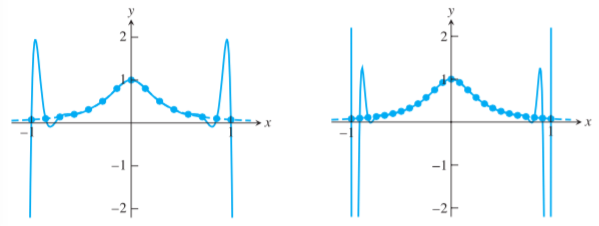
\includegraphics[width=9cm]{figs/3-2-3_Runge-1} 
\caption{左图为15个插值点的多项式插值;右图为25个插值点的多项式插值} 
\end{figure}
\end{frame}


\begin{frame}
\frametitle{Runge现象}
可以发现,多项式插值在区间的内部效果比较好,但是在靠近区间端点的地方出现了很大的波动。这种现象在高次多项式插值经常发生,被称为Runge现象。这种现象发生的原因可以通过插值误差观察出来,在插值误差公式中,一方面如果我们采取等距插值,即$x_{i+1} - x_i = x_{j+1} - x_j$,
\begin{equation}
\frac{(x - x_1)(x - x_2) \ldots (x-x_n)}{n!}
\end{equation}
在越靠近区间端点的地方绝对值越大,另一方面,即便是无穷可导的函数,其高阶导数$f^{(n)}(\xi)$并不一定性质非常好。因此,我们期望能够将插值点更多的移动到靠近插值区间端点的地方以解决这个问题。这就引出了Chebyshev插值。但其内容超出了本课程讨论的范围,有兴趣的同学可以阅读课本[NA]3.3章节。
\end{frame}


%%%%%%%%%%%%%%%%%%%%%%%%%%%%%%%%%%%%%%%%%%



\section{三次样条插值}

\begin{frame}
\frametitle{样条插值}
样条插值是插值的另一种方法。在多项式插值中,我们用一个多项式函数进行插值使得这个多项式函数经过所有的插值点,而这样的多项式会随着插值点的增加而逐渐变为高次多项式。在样条插值中,我们利用多个低次的多项式进行插值,使得这些多个低次多项式仍然经过给定的插值点。

\vspace{0.2cm}

最简单的样条插值就是线性样条插值,也就是将插值点$(x_1, y_1), \ldots, (x_n,y_n)$直接用直线连起来。例如对于插值点$(1,2), (2,1), (4,4), (5,3)$,利用线性样条插值得到的函数如下图
\begin{figure}
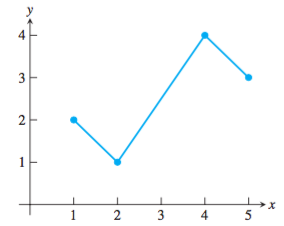
\includegraphics[width=4cm]{figs/3-4_Cubic_Splines-1} 
%\caption{$f(x) = x^3 + x -1$的图像} 
\end{figure}
\end{frame}


\begin{frame}
\frametitle{三次样条插值}
线性插值虽然可以让插值函数通过插值点,但是插值函数没有光滑性,也就是说插值函数没有连续的一阶、二阶导数。为此,我们可以利用三次样条插值,即我们用特定的三次函数来连接各插值点,并且通过一些条件使得插值函数在给定的插值区间上具有光滑性。例如对于插值点$(1,2), (2,1), (4,4), (5,3)$,利用三次样条插值得到的函数如下图
\begin{figure}
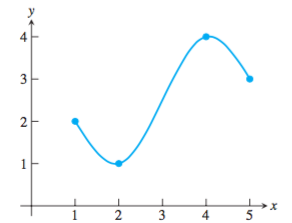
\includegraphics[width=4cm]{figs/3-4_Cubic_Splines-2} 
%\caption{$f(x) = x^3 + x -1$的图像} 
\end{figure}
\end{frame}


\begin{frame}
\frametitle{三次样条插值}
具体来说我们可以用待定系数的方式来求三次样条插值。例如,要求经过插值点$(x_1, y_1), \ldots, (x_n,y_n)$的三次样条插值$S(x)$,我们首先设在区间$[x_i, x_{i+1}]$上$S(x)$的表达式为$S_i(x)$,则$S_i(x)$为一个三次多项式且满足
\begin{enumerate}
\item $S_i(x_i) = y_i, \quad i = 1, \ldots, n-1$;
\item $S_i(x_{i+1}) = y_{i+1},  \quad i = 1, \ldots, n-1$ (以上两类条件相当于分段插值函数在插值节点上函数值相等);
\item $S'_{i-1}(x_i) = S'_i(x_i), \quad i = 2, \ldots, n-1$(在插值节点上一阶导数值相等);
\item $S''_{i-1}(x_i) = S''_i(x_i), \quad i = 2, \ldots, n-1$(在插值节点上二阶导数值相等)。
\end{enumerate}
由于$S(x)$在每个区间是三次多项式,因此二阶连续可导。
\end{frame}


\begin{frame}
\frametitle{三次样条插值}
根据上面的条件,我们可以设
\begin{align}
\label{eq: cubic spline formulation}
S_1(x) &= y_1 + b_1(x-x_1) + c_1 (x-x_1)^2 + d_1 (x-x_1)^3, \quad x \in [x_1, x_2], \nonumber \\
S_2(x) &= y_2 + b_2(x-x_2) + c_2 (x-x_2)^2 + d_2 (x-x_2)^3, \quad x \in [x_2, x_3], \nonumber \\
\vdots \nonumber \\
S_{n-1}(x) &= y_{n-1} + b_{n-1}(x-x_{n-1}) + c_{n-1} (x-x_{n-1})^2 + d_{n-1} (x-x_{n-1})^3, \nonumber \\
\quad &x \in [x_1, x_2].
\end{align}
这样假设$S(x)$的形式可以保证第一类条件自然的成立。之后我们希望利用第二、三、四类条件逐一把$b_i, c_i, d_i, i = 1, \ldots, n-1$求出来。但是我们看到,未知量$b_i, c_i, d_i$的个数是$3 \times (n-1) = 3n - 3$,而之前的二、三、四类条件给出的条件一共是$(n-1) + 2 \times (n-2) = 3n - 5$。也就是说,我们至少还需要增加两个条件才有可能将这些待定系数唯一的确定出来。
\end{frame}


\begin{frame}
\frametitle{三次样条插值}
我们发现,对于第三和第四类条件,即一阶和二阶导数的限制只存在于$i = 2, \ldots, n-1$的点上,因此我们可以在插值区间端点上,即$(x_1, y_1)$和$(x_n, y_n)$点上对插值函数的一阶或二阶导数值进行限制得到另外两个条件,进而将待定的系数唯一的确定出来。这里我们以比较常用的自然边界条件为例,推导如何得到样条插值的系数。首先我们有

\begin{definition}[自然边界条件]
对于三次样条插值,我们称
\begin{equation}
S_1''(x_1) = 0, \quad S''_{n-1}(x_n) = 0,
\end{equation}
为自然边界条件。
\end{definition}
\end{frame}


\begin{frame}
\frametitle{三次样条插值}
由$S_i(x)$的表达式,根据第二类的条件,我们有
\begin{align}
\label{eq: cubic spline system 1-1}
y_2 = S_1(x_2) = &y_1 + b_1(x_2-x_1) + c_1(x_2-x_1)^2 + d_1 (x_2-x_1)^3, \nonumber \\
\vdots \nonumber \\
y_n = S_{n-1}(x_n) = &y_{n-1} + b_{n-1}(x_{n}-x_{n-1}) + c_{n-1}(x_{n}-x_{n-1})^2 \nonumber \\
                                    &+ d_{n-1} (x_{n}-x_{n-1})^3.
\end{align}
\end{frame}


\begin{frame}
\frametitle{三次样条插值}
由$S_i(x)$的表达式,根据第三类的条件,我们有
\begin{align}
\label{eq: cubic spline system 2-1}
0 = S'_1(x_2) - S'_2(x_2) =& b_1 + 2c_1(x_2 - x_1) + 3d_1(x_2 - x_1)^2 - b_2, \nonumber \\
\vdots \nonumber \\
0 = S'_{n-2}(x_{n-1}) - S'_{n-1}(x_{n-1}) =& b_{n-2} + 2c_{n-2}(x_{n-1} - x_{n-2}) \nonumber \\
                                                                  & + 3d_{n-2}(x_{n-1} - x_{n-1})^2 - b_{n-1}. 
 \end{align}
\end{frame}


\begin{frame}
\frametitle{三次样条插值}
由$S_i(x)$的表达式,根据第四类的条件,我们有
\begin{align}
\label{eq: cubic spline system 3-1}
0 = S''_1(x_2) - S''_2(x_2) =& 2c_1 + 6 d_1 (x_2 - x_1) - 2c_2, \nonumber \\
\vdots \nonumber \\
0 = S''_{n-2}(x_{n-1}) - S''_{n-1}(x_{n-1}) =& 2c_{n-2} + 6 d_{n-2} (x_{n-1} - x_{n-2}) - 2c_{n-1}. 
 \end{align}
\end{frame}


\begin{frame}
\frametitle{三次样条插值}
我们可以利用方程组\eqref{eq: cubic spline system 1-1}, \eqref{eq: cubic spline system 2-1} , \eqref{eq: cubic spline system 3-1}以及自然边界条件得到系数$b_i, c_i, d_i$,但是直接解这$3n-3$个方程组成的方程组计算量比较大,我们采取解耦的方式来解这个方程组。

\vspace{0.2cm}

为此,我们令$\delta_i = x_{i+1} - x_i$,$\Delta_i = y_{i+1} - y_i$,然后将$c_i, i = 1, \ldots n-1$作为未知量,代入方程组\eqref{eq: cubic spline system 3-1}得
\begin{align}
\label{eq: d_i about c_i}
d_i = \frac{c_{i+1} - c_i}{3 \delta_i}, \quad i = 1, \ldots, n-2.
\end{align}
由将三次样条插值\eqref{eq: cubic spline formulation}的最后一个表达式求二阶导,我们有
\begin{equation}
d_{n-1} = \frac{\frac{S_{n-1}''(x_n)}{2}-c_{n-1}}{3} =:  \frac{c_n - c_{n-1}}{3\delta_{n-1}},
\end{equation}
其中我们令$c_{n} = \frac{S_{n-1}''(x_n)}{2}$。也就是说形式上\eqref{eq: d_i about c_i}对于$i = 1, \ldots, n-1$都成立,我们得到了$d_i$关于$c_i$的表达式。
\end{frame}


\begin{frame}
\frametitle{三次样条插值}
将$d$关于$c$的表达式代入到\eqref{eq: cubic spline system 1-1}并利用$\delta_i$和$\Delta_i$的定义,可以得到$b$关于$c$的表达式
\begin{align}
\label{eq: b_i about c_i}
b_i & = \frac{y_{i+1} - y_i}{x_{i+1} - x_i} - c_i (x_{i+1} - x_i) - d_i(x_{i+1} - x_i)^2 \nonumber \\
      & = \frac{\Delta_i}{\delta_i} - c_i \delta_i - \frac{\delta_i}{3}(c_{i+1} - c_i) \nonumber \\
      & = \frac{\Delta_i}{\delta_i} - \frac{\delta_i}{3}(2c_i + c_{i+1}), \quad i = 1, \ldots, n-1.
\end{align}
\end{frame}


\begin{frame}
\frametitle{三次样条插值}
最后将$b$和$d$关于$c$的表达式代入\eqref{eq: cubic spline system 2-1},得到
\begin{align}
\delta_1 c_1 + 2(\delta_1 + \delta_2) c_2 + \delta_2 c_3 &= 3(\frac{\Delta_2}{\delta_2} - \frac{\Delta_1}{\delta_1}) \nonumber \\
& \vdots \nonumber \\
\delta_{n-2} c_{n-2} + 2(\delta_{n-2} + \delta_{n-1}) c_{n-1} + \delta_{n-1} c_n &= 3(\frac{\Delta_{n-1}}{\delta_{n-1}} - \frac{\Delta_{n-2}}{\delta_{n-2}}).
\end{align}
同时根据自然边界条件以及\eqref{eq: cubic spline system 1-1}的第一个式子,我们有
\begin{align}
S''_1(x_1) = 0 \rightarrow 2c_1 = 0, \nonumber \\
S''_{n-1}(x_n) = 0 \rightarrow 2c_n = 0.
\end{align}
\end{frame}


\begin{frame}
\frametitle{三次样条插值}
我们可以将关于$c_1 , \ldots, c_n$的方程组写成矩阵形式
\begin{align}
&\left[ \begin{array}{cccccc}
     1                 & 0                             & 0                                      & 0                    &\ldots                                               & 0                \\  
     \delta_1      & 2\delta + 2\delta_2 & \delta_2                            & \ddots             & \vdots                                            & 0                \\ 
     0                 & \delta_2                  & 2\delta_2 + 2\delta_3       & \delta_3          & \ddots                                            & 0                \\
      \vdots        & \ddots                     &  \ddots                               &  \ddots            & \ddots                                           & \vdots         \\
      0                & \ldots                      & \ldots                                 &  \delta_{n-2}   & 2 \delta_{n-2} + 2\delta_{n-1}       & \delta_{n-1} \\
      0                & \ldots                      & \ldots                                 &  0                    & 0                                                  & 1                  \\      
       \end{array} \right] 
\left[ \begin{array}{c} 
      c_{1} \\ \quad \\ \quad \\ \vdots \\ \quad \\ c_n \end{array} \right] \nonumber \\
=&
\left[ \begin{array}{c}
     0 \\ 3(\frac{\Delta_2}{\delta_2} - \frac{\Delta_1}{\delta_1}) \\ \quad \\ \vdots \\ \quad \\ 3(\frac{\Delta_{n-1}}{\delta_{n-1}} - \frac{\Delta_{n-2}}{\delta_{n-2}}) \\ 0 \end{array} \right].
\end{align}
\end{frame}


\begin{frame}
\frametitle{三次样条插值}
我们发现,上面的方程组关于$c$存在唯一解,这是因为上面的方程组的系数矩阵是严格对角占优的。我们最后将$c$代入到$b$和$d$的表达式中得到各系数。

\begin{example}
找到过点$(0,3), (1,-2), (2,1)$的满足自然边界条件的三次样条插值。
\end{example}
根据之前的推导,我们有$\delta_1 = \delta_2 = 1$, $\Delta_1 = -5$, $\Delta_2 = 3$。从而我们得到关于$c$的方程组
\begin{align}
\left[ \begin{array}{ccc}
     1                 & 0                             & 0                                      \\  
     1      & 4 &1                            \\ 
     0                 &0                  & 1       \\    
       \end{array} \right] 
\left[ \begin{array}{c} 
      c_{1} \\ c_2\\ c_3 \end{array} \right] 
=
\left[ \begin{array}{c}
     0 \\ 24 \\ 0 \end{array} \right].
\end{align}
容易得到这个方程的解是$[c_1, c_2, c_3] = [0, 6, 0]$。利用\eqref{eq: d_i about c_i}和\eqref{eq: b_i about c_i},我们得到
\end{frame}


\begin{frame}
\frametitle{三次样条插值}
\begin{align}
d_1 = \frac{c_2 - c_1}{3 \delta_1} = 2, \quad d_2 = \frac{c_3 - c_2}{3 \delta_2} = -2,
\end{align}
以及
\begin{align}
b_1 = \frac{\Delta_1}{\delta_1}  - \frac{\delta_1}{3}(2c_1 + c_2) = -7, \quad b_2 = \frac{\Delta_2}{\delta_2}  - \frac{\delta_2}{3}(2c_2 + c_3) = -1.
\end{align}
因此,要求的三次样条插值为
\begin{align}
S_1(x) &= 3 - 7x + 0x^2 + 2x^3, \quad x \in [0,1], \nonumber \\
S_2(x) &= -2 -1(x-1) + 6(x-1)^2 - 2(x-1)^3, \quad x \in [1,2].
\end{align}
\end{frame}
%%%%%%%%%%%%%%%%%%%%%%%%%%%%%%%%%%%%%%%%%%

\begin{frame}
\frametitle{课后阅读及作业}
[NA] 第3章 3.1.1,3.1.2, 3.1.5, 3.2.1, 3.2.3,3.4.1 \\
作业:[NA] 3.1:1,2,12,13;3.2: 1,3,5;3.4:5,8,17。


\end{frame}

\end{document}

